\documentclass[handout]{ximera}


\graphicspath{  
{./}
{./whoAreYou/}
{./drawingWithTheTurtle/}
{./bisectionMethod/}
{./circles/}
{./anglesAndRightTriangles/}
{./lawOfSines/}
{./lawOfCosines/}
{./plotter/}
{./staircases/}
{./pitch/}
{./qualityControl/}
{./symmetry/}
{./nGonBlock/}
}


%% page layout
\usepackage[cm,headings]{fullpage}
\raggedright
\setlength\headheight{13.6pt}


%% fonts
\usepackage{euler}

\usepackage{FiraMono}
\renewcommand\familydefault{\ttdefault} 
\usepackage[defaultmathsizes]{mathastext}
\usepackage[htt]{hyphenat}

\usepackage[T1]{fontenc}
\usepackage[scaled=1]{FiraSans}

%\usepackage{wedn}
\usepackage{pbsi} %% Answer font


\usepackage{cancel} %% strike through in pitch/pitch.tex


%% \usepackage{ulem} %% 
%% \renewcommand{\ULthickness}{2pt}% changes underline thickness

\tikzset{>=stealth}

\usepackage{adjustbox}

\setcounter{titlenumber}{-1}

%% journal style
\makeatletter
\newcommand\journalstyle{%
  \def\activitystyle{activity-chapter}
  \def\maketitle{%
    \addtocounter{titlenumber}{1}%
                {\flushleft\small\sffamily\bfseries\@pretitle\par\vspace{-1.5em}}%
                {\flushleft\LARGE\sffamily\bfseries\thetitlenumber\hspace{1em}\@title \par }%
                {\vskip .6em\noindent\textit\theabstract\setcounter{question}{0}\setcounter{sectiontitlenumber}{0}}%
                    \par\vspace{2em}
                    \phantomsection\addcontentsline{toc}{section}{\thetitlenumber\hspace{1em}\textbf{\@title}}%
                     }}
\makeatother



%% thm like environments
\let\question\relax
\let\endquestion\relax

\newtheoremstyle{QuestionStyle}{\topsep}{\topsep}%%% space between body and thm
		{}                      %%% Thm body font
		{}                              %%% Indent amount (empty = no indent)
		{\bfseries}            %%% Thm head font
		{)}                              %%% Punctuation after thm head
		{ }                           %%% Space after thm head
		{\thmnumber{#2}\thmnote{ \bfseries(#3)}}%%% Thm head spec
\theoremstyle{QuestionStyle}
\newtheorem{question}{}



\let\freeResponse\relax
\let\endfreeResponse\relax

%% \newtheoremstyle{ResponseStyle}{\topsep}{\topsep}%%% space between body and thm
%% 		{\wedn\bfseries}                      %%% Thm body font
%% 		{}                              %%% Indent amount (empty = no indent)
%% 		{\wedn\bfseries}            %%% Thm head font
%% 		{}                              %%% Punctuation after thm head
%% 		{3ex}                           %%% Space after thm head
%% 		{\underline{\underline{\thmname{#1}}}}%%% Thm head spec
%% \theoremstyle{ResponseStyle}

\usepackage[tikz]{mdframed}
\mdfdefinestyle{ResponseStyle}{leftmargin=1cm,linecolor=black,roundcorner=5pt,
, font=\bsifamily,}%font=\wedn\bfseries\upshape,}


\ifhandout
\NewEnviron{freeResponse}{}
\else
%\newtheorem{freeResponse}{Response:}
\newenvironment{freeResponse}{\begin{mdframed}[style=ResponseStyle]}{\end{mdframed}}
\fi



%% attempting to automate outcomes.

%% \newwrite\outcomefile
%%   \immediate\openout\outcomefile=\jobname.oc
%% \renewcommand{\outcome}[1]{\edef\theoutcomes{\theoutcomes #1~}%
%% \immediate\write\outcomefile{\unexpanded{\outcome}{#1}}}

%% \newcommand{\outcomelist}{\begin{itemize}\theoutcomes\end{itemize}}

%% \NewEnviron{listOutcomes}{\small\sffamily
%% After answering the following questions, students should be able to:
%% \begin{itemize}
%% \BODY
%% \end{itemize}
%% }
\usepackage[tikz]{mdframed}
\mdfdefinestyle{OutcomeStyle}{leftmargin=2cm,rightmargin=2cm,linecolor=black,roundcorner=5pt,
, font=\small\sffamily,}%font=\wedn\bfseries\upshape,}
\newenvironment{listOutcomes}{\begin{mdframed}[style=OutcomeStyle]After answering the following questions, students should be able to:\begin{itemize}}{\end{itemize}\end{mdframed}}



%% my commands

\newcommand{\snap}{{\bfseries\itshape\textsf{Snap!}}}
\newcommand{\flavor}{\link[\snap]{https://snap.berkeley.edu/}}
\newcommand{\mooculus}{\textsf{\textbf{MOOC}\textnormal{\textsf{ULUS}}}}


\usepackage{tkz-euclide}
\tikzstyle geometryDiagrams=[rounded corners=.5pt,ultra thick,color=black]
\colorlet{penColor}{black} % Color of a curve in a plot



\ifhandout\newcommand{\mynewpage}{\newpage}\else\newcommand{\mynewpage}{}\fi


\title{Symmetries}
\author{Bart Snapp and Brad Findell}

\outcome{Learning outcome goes here.}

\begin{document}
\begin{abstract}
  We introduce symmetries.
\end{abstract}
\maketitle

\noindent\textbf{Group members (please print):}\ \hrulefill \\

\hrulefill
%% \begin{teachingnote}
%% An important learning challenge: The identity transformation (e.g., a $0^\circ$ or $360^\circ$ rotation) needs to be a symmetry of a figure so that the composition of two symmetries is also a symmetry of the figure.  More concretely, it would be strange for an equilateral triangle to have three reflection symmetries and only two rotational symmetries.
%% \end{teachingnote}

\begin{definition}
A symmetry is a transformation that takes a figure onto itself.  
\end{definition}
\begin{problem}
List the symmetries of an equilateral triangle.  Explain how you know you have them all.  
\end{problem}

\begin{problem}
Flip through these notes and describe the symmetries you notice.  Try to find reflection symmetry, rotation symmetry, and translation symmetry.  
\end{problem}

\begin{teachingnote}
To augment the examples, bring some pictures from Web.   Tesselations and Frieze patterns are necessary for translation symmetry.  
\end{teachingnote}

\begin{problem}
Suppose the symmetries of a square are called $R_0$, $R_{90}$, $R_{180}$, $R_{270}$, $V$, $H$, $D$, $D'$, based upon the figure below.  
\begin{image}
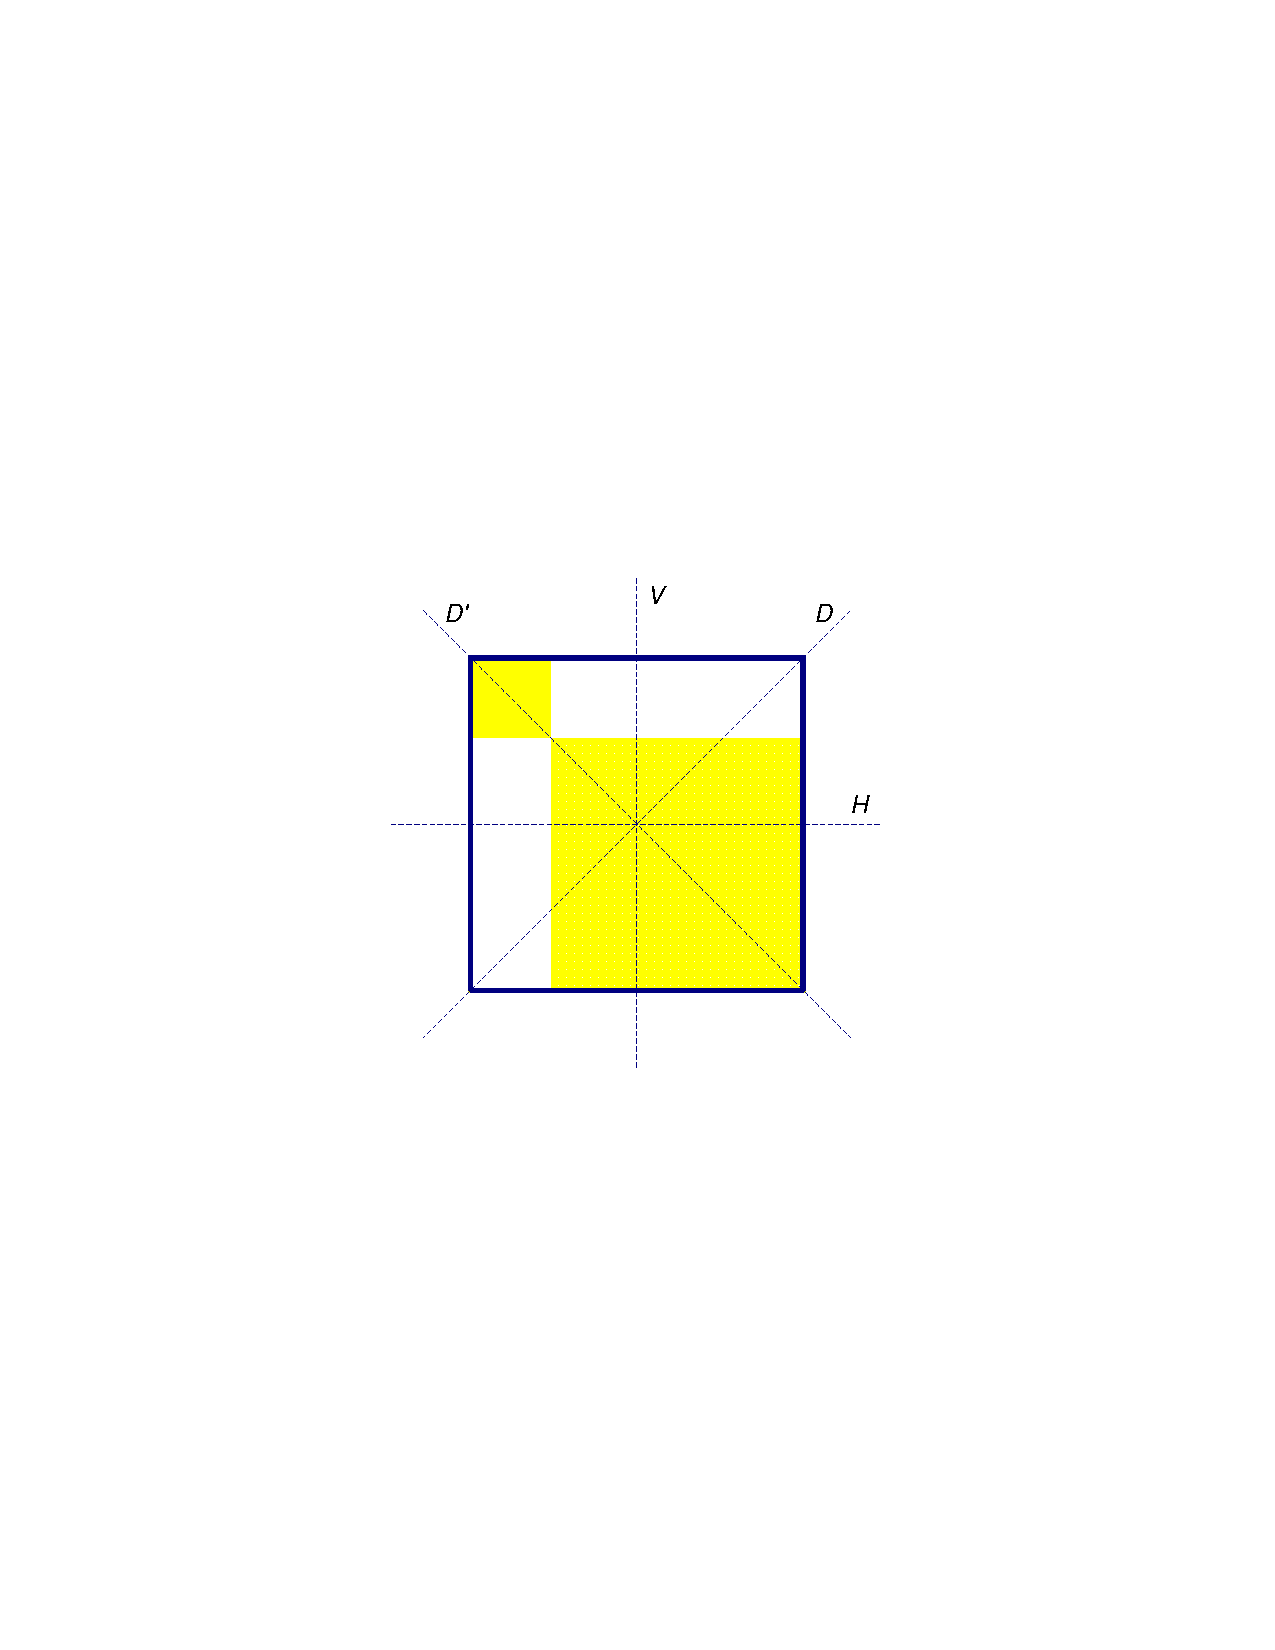
\includegraphics[scale=0.6]{D4.pdf}
\end{image}
Hint:  To identify a single transformation that accomplishes a sequence of transformations, do the transformations physically with a square piece of paper marked with ``FRONT'' on the side that starts facing you.  Or mark the corners of the square with $A$, $B$, $C$, and $D$.  
\begin{enumerate}
\item Complete the following table, where the entry at (row, column) is the symmetry that results from the sequence of symmetries given by the row heading followed by the column heading.  
\item What patterns and not-quite-patterns do you notice in the table?  For example, which elements ``commute'' with which other elements?
\item What facts about isometries can you observe in the table?  For example, what can you say generally about sequences of rotations and reflections?  
\end{enumerate}
\[
{\arraycolsep=12pt\def\arraystretch{3}
\begin{array}{|l||l|l|l|l||l|l|l|l|}
\hline
 & R_0 & R_{90} & R_{180} & R_{270} & V & H & D & D' \\ \hline\hline
R_0 & & & & & & & & \\ \hline
R_{90} & & & & & & & & \\ \hline
R_{180} & & & & & & & & \\ \hline
R_{270} & & & & & & & & \\ \hline\hline
V & & & & & & & & \\ \hline
H & & & & & & & & \\ \hline
D & & & & & & & & \\ \hline
D' & & & & & & & & \\ \hline
\end{array}
}\]
\end{problem}

%% \begin{teachingnote}
%% Blurring one's eyes, it is possible to notice (1) the composition of a reflection and a rotation (in either order) is a reflection; (2) the composition of two rotations is a rotation; and (3) the composition of two reflections is a rotation.  Looking a bit closer, one can see that some elements commute with one another and others do not.  
%% \end{teachingnote}
\end{document}
